\section{Robustness measures and uncertainty thresholding}
\label{sec: robustness measures}

%\rednote{ACTUALLY I THINK THIS SHOULD GO IN FRONT OF THE BIAS CORRECTION SECTION?} maybe. Might be worth rethinking about how to structure the paper honestly. 
In this section, we introduce a unified statistic $\hat{E}$ for evaluating the total error in an approximated posterior. From this discussion, the concepts of accuracy and precision for posterior estimators naturally appear. We also define the accuracy statistic $\hat{A}$ and precision statistic $\hat{\Pi}$ for estimating these quantities, where the error statistic is the sum $\hat{E} = \hat{A} + \hat{\Pi}$. We note that the precision statistic is proportional to the doubly-integrated Eq. A10 from \citet{Essick:2022ojx}.

To quantify the error between the posterior estimator and the true posterior, we use the \KL divergence. Given a reference probability distribution $p$ and a test distribution $q$ over a space $\Lambda$, the \KL divergence quantifies the information lost from approximating $p$ with $q$. In units of bits \citep{MacKay2003}
\beq
\KLD(p|q) = \int p(\Lambda) \log_2\left(\frac{p(\Lambda)}{q(\Lambda)}\right)\dd\Lambda.
\label{eq: kl divergence}
\eeq
Suppose $q(\Lambda) \propto p(\Lambda)(1+\delta(\Lambda))$ for a small perturbation function $\delta(\Lambda)$. Expanding the logarithm and ensuring $q(\Lambda)$ is normalized gives\footnote{We can also think of Eq.~\ref{eq: kl divergence at leading order} as a different quantification for the distance between distributions: the $L^2$ norm of the centralized perturbation function $||\delta(\Lambda) - \int p(\Lambda')\delta(\Lambda')\dd\Lambda'||^2$ on the probability space defined by $p(\Lambda)$. This metric (which approximates the \KL divergence) is zero if and only if $\delta(\Lambda)-\int p(\Lambda')\delta(\Lambda')\dd\Lambda' = 0$ over the entire support of $p$.}
\beq
\KLD(p|q) \approx \frac{1}{2\ln(2)} \left[\int p(\Lambda)\delta(\Lambda)^2\dd\Lambda - \left(\int p(\Lambda)\delta(\Lambda)\dd\Lambda\right)^2\right] + \mathcal{O}(\delta^3).
\label{eq: kl divergence at leading order}
\eeq

Here, $p$ represents the true posterior and $q=\hat{p}$ the estimator, and so $\delta(\Lambda) = b(\Lambda) + \varepsilon(\Lambda)$ is the sum of a constant bias term $b(\Lambda)$ (defined in Eq.~\ref{eq: posterior bias}) and a (zero mean) scatter term $\varepsilon(\Lambda)$. Taking the expectation of both sides and using that $\expect{\varepsilon(\Lambda)} = 0$, $\expect{\varepsilon(\Lambda)\varepsilon(\Lambda')} = C_{\ln\mathcal{L}}(\Lambda, \Lambda')$ and $C_{\ln\mathcal{L}}(\Lambda, \Lambda) \equiv \sigma^2_{\ln\mathcal{L}}(\Lambda)$
\beq
\expect{\KLD(p|\hat{p})} \approx \frac{1}{2\ln(2)} \left[\int p(\Lambda)[b(\Lambda)^2 + \sigma^2_{\ln\mathcal{L}}(\Lambda)]\dd\Lambda - \int p(\Lambda)p(\Lambda')[b(\Lambda)b(\Lambda') + C_{\ln\mathcal{L}}(\Lambda,  \Lambda')]\dd\Lambda\dd\Lambda'\right] + \mathcal{O}(\delta^3).
\label{eq: expected kl divergence to estimator}
\eeq
This motivates the definition of the error statistic $\hat{E}$, which estimates Eq.~\ref{eq: expected kl divergence to estimator}. Given $N_{\rm samp}$ samples $\{\Lambda_n\}$ from the hyperposterior estimator $\hat{p}$, we define the error statistic as 
\beq
\hat{E}[\hat{p}] = \hat{A}[\hat{p}] + \hat{\Pi}[\hat{p}]
\label{eq: error statistic}
\eeq
where $\hat{A}$ estimates the terms containing the bias $b(\Lambda)$, and so the overall effect of the bias in the posterior, and $\hat{\Pi}$ estimates the uncertainty, 
\begin{align}
    \hat{\Pi}[\hat{p}] &= \frac{1}{2\ln(2)}\left[\frac{1}{N_{\rm samp}}\sum_{n=1}^{N_{\rm samp}}\hat{\sigma}^2_{\ln\mathcal{L}}(\Lambda_n) - \frac{1}{N_{\rm samp}^2}\sum_{n=1}^{N_{\rm samp}}\sum_{m=1}^{N_{\rm samp}}\hat{C}_{\ln\mathcal{L}}(\Lambda_n, \Lambda_m)\right]
    \label{eq: precision statistic} \\
    \hat{A}[\hat{p}] &= \frac{1}{2\ln(2)}\frac{1}{N_{\rm samp}-1}\left[\sum_{n=1}^{N_{\rm samp}}\bar{K}_{\ln\mathcal{L}}(\Lambda_n)^2 - \frac{1}{N_{\rm samp}}\left(\sum_{n=1}^{N_{\rm samp}}\bar{K}_{\ln\mathcal{L}}(\Lambda_n)\right)^2\right] = \frac{1}{2\ln(2)}{\rm var}[\{\bar{K}_{\ln\mathcal{L}}(\Lambda_n)\}],
    \label{eq: accuracy statistic}
\end{align}
and $\hat{\sigma}^2_{\ln\mathcal{L}}(\Lambda_n)\equiv\hat{C}_{\ln\mathcal{L}}(\Lambda_n, \Lambda_n)$ is the estimator of the variance of the log-likelihood defined in Eq.~\ref{eq: likelihood variance estimator}, $\hat{C}_{\ln\mathcal{L}}(\Lambda_n, \Lambda_m)$ is the estimator for the covariance of the log-likelihood between points $\Lambda_n$ and $\Lambda_m$ defined in Eq.~\ref{eq: population covariance with selection}, and the weights are given by
\beq
\bar{K}_{\ln\mathcal{L}}(\Lambda_n) = 
\begin{cases}
\dfrac{1}{2}\dfrac{\Nobs(\Nobs+1)\hat{\sigma}^2_{\xi}(\Lambda_n)}{\hat{\xi}(\Lambda_n)^2} - \dfrac{1}{N_{\rm samp}}\displaystyle\sum_{m=1}^{N_{\rm samp}} \hat{C}_{\ln\mathcal{L}}(\Lambda_n, \Lambda_m) & \text{if using uncorrected likelihood (Eq.~\ref{eq: estimated hierarchical likelihood})} \\ 
\dfrac{1}{N_{\rm samp}}\displaystyle\sum_{m=1}^{N_{\rm samp}} \hat{C}_{\ln\mathcal{L}}(\Lambda_n, \Lambda_m)  & \text{if using corrected likelihood (Eq.~\ref{eq: unbiased likelihood estimator})}
\end{cases}
\label{eq: weights for computing accuracy}
\eeq
where the sum estimates the average covariance between the fixed point $\Lambda_n$ and another random sample in the posterior $\hat{p}$. 

The accuracy statistic $\hat{A}[\hat{p}]$ approximates the amount of bias in the posterior estimate $\hat{p}$ from the true posterior $p$. Given that we do not have access to an ensemble of posterior estimators nor the true posterior, we can only estimate the bias to leading order. We neglect the higher order terms that should also contribute to the accuracy. A large accuracy statistic indicates that higher order terms would also contribute significantly to the bias, and the posterior estimator is not trustworthy. 

Similarly, the precision statistic $\hat{\Pi}[\hat{p}]$ measures the average amount of scatter in a theoretical ensemble of posterior estimators. The scatter is the distance between the average posterior estimator (which in general is biased from the true posterior) and the particular realization of the posterior estimator. Again, we do not have access to this theoretical ensemble, and so we can only estimate the precision to leading order based on the estimator we have. 
We verify the efficacy of the accuracy and precision statistics for a variety of hierarchical inference problems in Sections~\ref{sec: gaussian example} and \ref{sec: gw example}. 
Additionally, note that the precision statistic is also proportional to the average variance in the difference of the log-likelihoods for two draws from the hyperposterior, discussed in \citet{Essick:2022ojx} and shown in Eq. A11 therein for the single-event terms.

For a variety of problems we consider, we find that when $\hat{E}[\hat{p}] \lesssim 0.2$ bits, the posterior estimator is reliable, and the smaller the error statistic, the more reliable the posterior estimator is. See Fig.~\ref{fig: accuracy vs precision} for a schematic to illustrate the concepts of accuracy and precision in a posterior estimator.

\begin{figure}
    \centering
    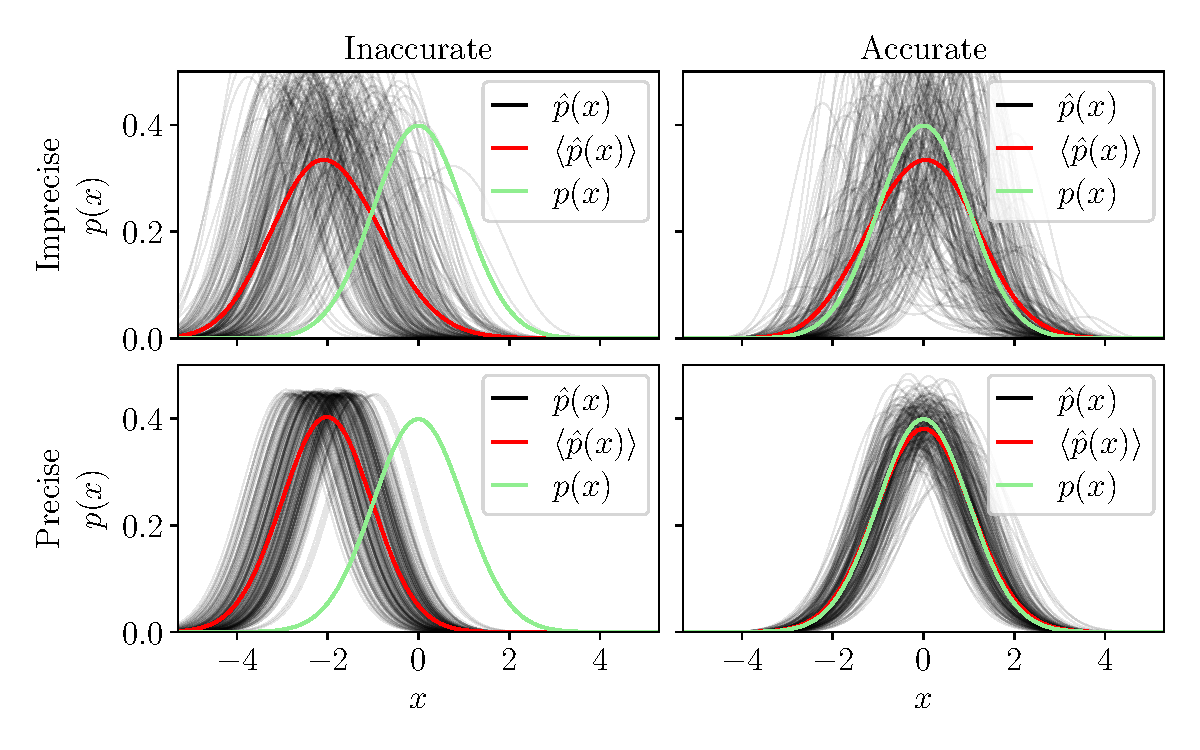
\includegraphics[width=0.8\linewidth]{plots/precision_vs_accuracy.pdf}
    \caption{Schematic showing the concept of precise and accurate posterior estimators. In all panels the black traces are draws from the posterior estimator $\hat{p}(x)$, the red curve is the mean of the posterior estimators, $\langle \hat{p}(x)\rangle$, and the green is the true posterior. \textit{Top left}: draws from an inaccurate, imprecise posterior estimator. The posterior estimators are inaccurate because the mean $\langle \hat{p}(x)\rangle$ posterior is significantly different from the true posterior $p(x)$, and the estimator is imprecise due to the large scatter around the true posterior. \textit{Top right}: the same as the top left, but with an accurate but imprecise posterior estimator. \textit{Bottom left}: draws from an inaccurate yet precise posterior estimator. \textit{Bottom right}: draws from an accurate and precise posterior estimator.}
    \label{fig: accuracy vs precision}
\end{figure}

Notice that the accuracy statistic is on the order of the \textit{square} of the covariance estimator and the precision is on the order of covariance estimator. As the uncertainty in the log-likelihood estimator decreases, the error is dominated by the uncertainty rather than the bias. In practice, though, there are scenarios where the bias can dominate the overall error. Bias and uncertainty in the estimator are due to different aspects of the ``noise process'' in the likelihood estimator. The bias in the posterior happens due to a changing variance/covariance across the support of the posterior, while the uncertainty in the posterior estimator comes from a variance in the log-likelihood estimator which is not matched by equal \textit{covariance} across the posterior support.

% We derive a pair of quantities to measure the accuracy and precision of a given posterior estimator. The accuracy statistic $\hat{A}$ \rednote{notation good?} we derive is directly related to the bias we discuss in detail above -- it represents the similarity between the \textit{average} posterior estimator and the true posterior (e.g. the difference between the red contour and the green contour in Figs.~\ref{fig: nobs 100 gaussian example} and \ref{fig: nobs 1000 gaussian example}). In practice, of course, we cannot calculate this exactly, however we can estimate it to leading order. 

% In addition to the accuracy of the posterior point estimate, there is the random scatter from using a single uncertain approximation to the posterior. We quantify this with a \textit{precision} statistic $\hat{\Pi}$ which measures the information lost -- on average -- between the a point estimate posterior estimator and the average posterior estimator (e.g. the difference between a black contour and the red contour in Figs.~\ref{fig: nobs 100 gaussian example} and \ref{fig: nobs 1000 gaussian example}).

% These are different but related issues associated with using an uncertain approximation for the likelihood. In different cases, posterior estimators may be both accurate and precise, accurate but imprecise, inaccurate but precise, or neither accurate nor precise. We show a simple schematic in Fig.~\ref{fig: accuracy vs precision}, and discuss the accuracy and precision statistics below.

% \subsection{Accuracy}

% For likelihoods with a large uncertainty, the posterior estimator can have a significant bias. We derived a general expression for the leading-order bias in Eq.~\ref{eq: full bias} -- which may be corrected with Eq. ????? -- and in the \ac{GW} population inference problem it's 
% \beq
% b(\Lambda) = \frac{1}{2}\frac{\Nobs(\Nobs+1)\hat{\sigma}_\xi^2(\Lambda)}{\hat{\xi}(\Lambda)^2} - \int \hat{C}_{\ln\mathcal{L}}(\Lambda, \Lambda')p(\Lambda')d\Lambda'
% \label{eq: bias in gw inference}
% \eeq
% \rednote{Now the left hand side $b(\Lambda)$ is not an estimator, but the RHS is an estimator. We should correct this -- ie write in terms of the true $C_{\ln\mathcal{L}}(\Lambda, \Lambda')$ which we argue can then be \textit{estimated} using the estimators.}
% where
% \beq
% \hat{\sigma}^2_\xi = \frac{1}{\Ninj-1}\left(\frac{1}{\Ninj}\sum_{j=1}^{\Ninj}\frac{p(\theta_j|\Lambda)^2}{p(\theta_j|{\rm draw})^2} - \hat{\xi}(\Lambda)^2\right)
% \eeq
% and
% \begin{multline}
% \hat{C}_{\ln\mathcal{L}}(\Lambda, \Lambda') = \sum_{i=1}^{\Nobs}\frac{1}{\NPE - 1}\frac{1}{\hat{p}(d_i|\Lambda)\hat{p}(d_i|\Lambda')}\left(\left[\frac{1}{\NPE}\sum_{j=1}^{\NPE}\frac{p(\theta_j|\Lambda)}{\pi(\theta_j|{\rm PE})}\frac{p(\theta_j|\Lambda')}{\pi(\theta_j|{\rm PE})}\right] - \hat{p}(d_i|\Lambda)\hat{p}(d_i|\Lambda')\right) \\
% + \frac{\Nobs^2}{\Ninj - 1}\frac{1}{\hat{\xi}(\Lambda)\hat{\xi}(\Lambda')}\left(\left[\frac{1}{\Ninj}\sum_{j=1}^{\Nfound}\frac{p(\theta_j|\Lambda)}{p(\theta_j|{\rm draw})}\frac{p(\theta_j|\Lambda')}{p(\theta_j|{\rm draw})}\right] - \hat{\xi}(\Lambda)\hat{\xi}(\Lambda')\right).
% \label{eq: gw posterior covariance} 
% \end{multline}
% Even including the likelihood unbiasing term, there is a residual bias in the posterior which can only be removed by redoing the analysis with a correction term derived from the initial biased inference. However, we can approximate the information lost (by manner of a \ac{KL} divergence) with Eq.~\ref{eq: kl divergence at leading order} for $\delta$, and therefore we get 
% \beq
% \KLD(p|\langle\hat{p}\rangle) = \frac{1}{2\ln(2)}\left[\int p(\Lambda)b(\Lambda)^2d\Lambda - \left(\int p(\Lambda) b(\Lambda)d\Lambda\right)^2\right] + \mathcal{O}(b^3)
% \eeq
% We can estimate this with an \textit{accuracy} statistic. 
% Given $N_{\rm samp}$ samples $\{\Lambda_n\}$ from the hyperposterior estimator $\hat{p}$, we define the accuracy statistic as
% \beq
% \hat{A}[\hat{p}] = \frac{1}{2\ln(2)}\mathbb{V}[\{\bar{K}_{\ln\mathcal{L}}(\Lambda_n)\}_{n=1}^{N_{\rm samp}}\}] \approx \KLD(p|\langle\hat{p}\rangle)
% \eeq
% where $\mathbb{V}$ denotes the sample variance in the set of weights 
% \beq
% \bar{K}_{\ln\mathcal{L}}(\Lambda_n) = \frac{1}{N_{\rm samp}}\sum_{m=1}^{N_{\rm samp}} \hat{C}_{\ln\mathcal{L}}(\Lambda_n, \Lambda_m).
% \eeq
% The $n^{\rm th}$ weight corresponds to the covariance between the point $\Lambda_n$ and another random sample from the hyperposterior $\Lambda_m \sim \hat{p}$, averaged over random samples $\Lambda_m$. Note the covariance is symmetric in $\Lambda_n \leftrightarrow \Lambda_m$, and so the weights may be equivalently computed as an average over the first argument or the second argument in the covariance.

% The accuracy statistic can be computed in post-processing after a stochastic sampler finishes producing the samples $\{\Lambda_n\} \sim \hat{p}$. \rednote{Ok so we should remove the likelihood biasing term! Just makes everything easier.}

% \subsection{Precision}

% \rednote{These should all have integration measure $\Lambda$}

% In addition to the bias discussed in Section~\ref{sec: monte carlo bias}, there is the uncertainty associated with using a single point estimate of the posterior. We can quantify this with Eq.~\ref{eq: kl divergence at leading order}, by taking the expectation over all $\delta$. This obtains us the \textit{precision} of the posterior estimator 
% \beq
% \langle\KLD(\langle \hat{p}\rangle|\hat{p})\rangle \approx \frac{1}{2\ln(2)} \left[\int p(x)\sigma^2(x)dx - \int p(x)p(x')C_{\ln\mathcal{L}}(x, x')dxdx'\right],
% \label{eq: random kl divergence expectation}
% \eeq
% where $C_{\ln\mathcal{L}}(x,x') = \langle\delta(x)\delta(x')\rangle$ is the covariance between two points $x, x'$ and $\sigma^2(x) = C_{\ln\mathcal{L}}(x,x)$.
% This is useful because we can also estimate this for an analysis without knowing the true posterior or the average of many posteriors. Given our single point estimate of the posterior $\hat{p}$, we define the \textit{precision} statistic as \rednote{we can create an accuracy estimator too based on the bias.}
% \beq
% \widehat{\Pi}[\hat{p}] = \frac{1}{2\ln(2)} \left[\int \hat{p}(x)\hat{\sigma}^2(x)dx - \int \hat{p}(x)\hat{p}(x')\hat{C}_{\ln\mathcal{L}}(x, x')dxdx'\right],
% \label{eq: precision estimator}
% \eeq
% \rednote{Write this in terms of samples and weights and shit, as done for the accuracy estimator.}


% where $\hat{\sigma}^2(x)$ is the estimator for the variance in the log-likelihood at the point $x$, and $\hat{C}_{\ln\mathcal{L}}(x,x')$ is the estimator for the covariance between the log-likelihood estimates at $x$ and $x'$. The precision statistic approximates the \textit{typical} amount of information lost from the the average posterior, when using a point estimate. It does not account for the additional bias that may be present in the average posterior. 

\subsection{Thresholding on the uncertainty}

Another perspective on the error in the posterior estimator is as a sum of contributions which occur at higher and higher order in the uncertainty of the log-likelihood. The leading order contribution to the error is the precision statistic, which occurs at first order in the covariance of the log-likelihood $C$. The bias occurs at order $C^2$, and in principle, there are contributions at third, fourth, etc. order in the covariance.\footnote{At higher order, there are also higher order moments which contribute, e.g. $\expect{\varepsilon(\Lambda)\varepsilon(\Lambda')\varepsilon(\Lambda'')}$, which must be accounted for.} 
However we neglect these to describe only the leading order contribution of the precision and the accuracy. If we bound the covariance to be below 1, that bounds the leading order sources of error and also ensures that the contributions at high order in the covariance are suppressed.

Fortunately, the covariance in the log-likelihood must satisfy
\beq
|C_{\ln\mathcal{L}}(\Lambda, \Lambda')| \le \sqrt{|C_{\ln\mathcal{L}}(\Lambda, \Lambda)||C_{\ln\mathcal{L}}(\Lambda', \Lambda')|} \equiv \sigma_{\ln\mathcal{L}}(\Lambda)\sigma_{\ln\mathcal{L}}(\Lambda'),
\label{eq: covariance Schwarz inequality}
\eeq
due to the Cauchy-Schwarz inequality, where $\sigma_{\ln\mathcal{L}}(\Lambda)$ is the square root of the variance of the log-likelihood estimator. The same inequality holds for the covariance and variance \textit{estimators}
\beq
|\hat{C}_{\ln\mathcal{L}}(\Lambda, \Lambda')| \le \hat{\sigma}_{\ln\mathcal{L}}(\Lambda)\hat{\sigma}_{\ln\mathcal{L}}(\Lambda').
\label{eq: covariance Schwarz inequality estimator}
\eeq
Showing these inequalities does require some careful application of the Cauchy-Schwarz inequality, which we do in Appendix~\ref{app: covariance cauchy-Schwarz}.

If we require that the variance in the log-likelihood estimator be bounded below some value (e.g. below 1, as recommended by \citet{Talbot:2023pex}), then this shows that the leading order contributions to error in the posterior estimators are bounded. Now, we do not have access to the true variance of the log-likelihood estimator, but we do have access to an estimator of the variance of the log-likelihood. We can cut out regions of $\Lambda$ parameter space wherever our estimator of the variance in the log-likelihood exceeds 1, and we show here that this bounds the error in the posterior estimator.\footnote{The uncertainty in the estimator for the variance in the log-likelihood is typically negligible, especially when the variance estimator itself is below 1.} This verifies the conjectured threshold on the log-likelihood put forth by \citet{Talbot:2023pex}.\footnote{That being said, there are pathological examples where this argument breaks down: for example, the arguments here fail if the likelihood does not admit a Taylor expansion.}

Using the above inequalities of Eqs.~\ref{eq: covariance Schwarz inequality} and \ref{eq: covariance Schwarz inequality estimator}, and a variance threshold $\sigma^2_{\rm MAX}$, the precision, accuracy and error statistics are bounded by 
\beq
\hat{\Pi}[\hat{p}] \le \frac{\sigma^2_{\rm MAX}}{\ln(2)} \qquad \qquad \hat{A}[\hat{p}] \le \frac{\sigma^4_{\rm MAX}}{2\ln(2)} \qquad \qquad \hat{E}[\hat{p}] \le \frac{\sigma^2_{\rm MAX}}{\ln(2)} + \frac{\sigma^4_{\rm MAX}}{2\ln(2)} 
\label{eq: error statistics bounds}
\eeq
but in practice tend to be much smaller than these bounds (typically by an order of magnitude or so).

While we show the log-likelihood variance threshold suggested in \citet{Talbot:2023pex} guarantees a trustworthy posterior estimator, it only does so within the domain of $\Lambda$ which is not below the variance threshold. Furthermore, \citet{Essick:2022ojx} point out that a threshold on the log-likelihood variance might be sufficient for accurate inference, but also that there are cases where thresholding on the log-likelihood variance is much stronger than necessary; these are the cases where we believe the error statistic is useful (\citet{Essick:2022ojx} and \citet{Talbot:2023pex} come to similar conclusions and define a statistic similar to our precision statistic). We discuss examples of the variance threshold being stronger than necessary in Section~\ref{sec: gw example}.

Another common threshold previously used in the literature is based on the effective sample size of a Monte Carlo integral. Somewhat confusingly, there are two related but subtly different definitions of the effective sample size, both of which are used. One definition, defined in \citet{Farr:2019rap}, is commonly applied to the selection efficiency Monte Carlo integral
\beq
N_{{\rm eff}, \xi} \equiv \frac{\hat{\xi}^2}{\hat{\sigma}_{\xi}^2}.
\eeq
\citet{Farr:2019rap} point out that, when $N_{{\rm eff}, \xi} < 4\Nobs$, then the likelihood estimator is extremely biased and so is almost certainly unreliable. However, the converse is not necessarily true: if $N_{{\rm eff},\xi} > 4\Nobs$ it is still possible that the likelihood estimator is too uncertain to be trusted. Indeed, the variance in the log-likelihood due to the selection efficiency Monte Carlo integral is $\Nobs^2 / N_{{\rm eff},\xi}$, and so for $\Nobs \gg 4$, we can have a large effective sample size, but a variance which is much larger than one, with no \textit{guarantee} that the posterior estimator is reliable (only the lack of a guarantee that the posterior estimator is \textit{not} reliable).


Historically, some of the first problems due to single-event Monte Carlo integrals (eq.~\ref{eq: single event estimator}) were encountered by \citet{KAGRA:2021duu}. To handle such issues, another definition of effective sample size due to \citet{kish1965survey} was used to ensure convergence, where
\beq
N_{{\rm eff}, p} \equiv \frac{\left(\sum_{j=1}^{\NPE} w_j\right)^2}{\sum_{j=1}^{\NPE} w_j^2} = \frac{\hat{p}^2}{\hat{\sigma}^2_{p} + \hat{p}^2/(\NPE-1)} \qquad\qquad \mathrm{where} \qquad \qquad w_j = \frac{p(\theta_j | \Lambda)}{\pi(\theta_j|{\rm PE})}.
\eeq
The threshold used by \citet{KAGRA:2021duu} was to require that \textit{all} single-event Monte Carlo integrals satisfy $N_{{\rm eff}, p} > \Nobs$. Other analyses have used different thresholds, requiring instead that $N_{{\rm eff}, p} > 10$ or some other fixed number. 
In particular, the thresholds we refer to as ``effective sample size'' or ``$\Neff$'' thresholds are
\begin{enumerate}
    \item $N_{{\rm eff},\xi} > 4\Nobs$
    \item $N_{{\rm eff},p} > 10, 30, \Nobs$ depending on the analysis threshold.
\end{enumerate}
Our claim is that these thresholds are not enough to ensure a reliable posterior estimator. Though these may produce reasonable results in some applications, we do not have any theoretical guarantee of reliable results, and we show examples in Section~\ref{sec: gw example} where these thresholds can be insufficient.
